\documentclass[12pt]{article}
\usepackage{graphicx} % Required for inserting images

\title{Lab 5: Digital Electronics Acquisition and Demonstration of Compton Scattering}
\author{Owen Strong \\
\itshape Prof.: Angela DiFulvio\\
\itshape TA: Kholod Mahmoud \\
\itshape TA: Shaffer Bauer \\
\itshape TA: Justin Jia \\
}
\date{March 8, 2026 (Adjusted from March 7)}

\usepackage[
    style=ieee
]{biblatex}
\bibliography{refs.bib}

\usepackage[letterpaper, margin=1in]{geometry}
\usepackage{xspace}

% Figure Macros
\newcommand{\figwidth}{0.75\linewidth}
\newcommand{\figref}[1]{Fig.~\ref{#1}}
\newcommand{\defplotW}[3]{
    \begin{figure}[!htb]
        \centering
        \includegraphics[width=#3\linewidth]{fig/#1.png}
        \caption{#2}
        \newcommand{\tmplabel}{fig:#1}
        \label{\tmplabel}
    \end{figure}
}
\newcommand{\defplot}[2]{\defplotW{#1}{#2}{0.75}}

% Common Macros
\newcommand{\micCi}{$\mathrm{\mu Ci}$\xspace}
\newcommand{\CsSrc}{$\mathrm{^{137}Cs}$\xspace}
\newcommand{\degr}{$^\circ$\xspace}

\usepackage{placeins} % FloatBarrier
\usepackage{amsmath} % align
\usepackage{xcolor}
\usepackage[colorlinks=true, citecolor=violet, linkcolor=violet, urlcolor=violet]{hyperref}
\usepackage{enumitem}

\begin{document}
\pagenumbering{gobble}
\maketitle
\pagebreak
{\hypersetup{linkcolor=black}\tableofcontents}
\pagebreak
\pagenumbering{arabic}
\begin{abstract}
    A key aspect of gamma ray interaction with matter is Compton scattering, the primary interaction for low-z materials like organics, in which an incident photon elastically scatters off of a discharged electron, the energies of which can be modeled kinematically.
    In this laboratory, we investigate the validity of the kinematic model of Compton scattering, using digitally acquired time-coincident measurements from two detectors.\\
    
    We measured energy spectra of responses to a 30~\micCi \CsSrc gamma source, by a stilbene organic scintillator and a NaI(Tl) inorganic scintillator, to calibrate energy spectra measurements using these detectors.
    We collimated the source with lead bricks and configured the organic and inorganic detectors to measure Compton scattering in the organic detector, with Compton electron energies measured by the organic detector, and deflected photons striking the inorganic detector (positioned at specific angles of 0, 30, 60, and 90~degrees), with a fast digitizer to record only simultaneous (within a window of 96~ns) responses from both detectors and thus primarily observe scattering events at these angles.\\

    We estimated calibration coefficients of 0.252~keV per channel for the inorganic detector, and 1.92~keV per channel for the organic detector.
    Using these coefficients, we compared the peak energy response from both detectors at different angles, and found that the peak responses from the organic detector roughly corresponded to the predicted Compton electron energy for each angle, while those from the inorganic detector roughly corresponded to the predicted scattered gamma ray energy for each angle.\\

    These results lend credence to the kinematic model of Compton scattering, insofar as to predict scattered particle energies, and additionally demonstrate the utility of the fast digitizer, and direct digital acquisition in general, through the effectiveness of time-coincidence filtering to isolate readings corresponding to different angles, and will be useful to those intending to use the kinematic model of Compton scattering, or those considering the use of direct digital acquisition, such as to take time-coincident measurements.

\end{abstract}

\section{Introduction and Background}

Gamma radiation interacts with matter through three primary mechanisms: photoelectric effect, Compton scattering, and pair production.\\

In the photoelectric effect, relevant for lower gamma energy and high-z atoms, photons are absorbed by an electron, dislodging it from the atom.
In pair production, relevant for high photon energy (specifically, greater than 1.022~MeV, twice the rest mass energy of an electron) the gamma ray strikes an atom with enough energy to produce a pair of an electron and positron, which quickly annihilate.
Finally, in Compton scattering, the photon and electron elastically scatter off of each other.
While Compton scattering can take place at any incident photon energy, it is most significant in the intermediate energies between where photoelectric effect and pair production dominate, and especially for lower-z atoms like the carbon, and hydrogen of organic materials, where neither photoelectric or pair production effects dominate, as seen in \figref{fig:intr0_effects}.\\

\defplotW{intr0_effects}{Regions of photon energy $\bar{h}\omega$ and target proton count where different photon interactions with matter tend to occur. Sourced from Nuclear Radiation Interactions (Second Edition)\cite{yip_nuclear_2025}}{0.6}

Compton scattering can be modeled kinetically, as shown in \figref{fig:intr1_kine}, in which the model of an elastic collision, accounting for relativistic behavior, predicts energies based on deflection angle $\theta$.
Electron binding energy is typically low enough to be ignored in this model.\\

\defplotW{intr1_kine}{Kinematics of Compton scattering, in which an incident photon of energy $E$ interacts with an electron at rest, with the photon scattering at angle $\theta$ to a lower energy $E'$ and transferring $E_e=E-E'$ to the ejected electron.}{0.6}


In this laboratory, we perform time-coincidence measurements using two detectors to compare energies of Compton scattered electrons and photons at different angles to verify theoretical Compton scattering kinematics.
In doing so, we also aim to demonstrate the use of direct digital acquisition electronics.
% Photoelectric effect
\subsection{Compton Kinematics}
% ...
Using conservation of energy $E_\gamma=E_\gamma'+E_e$ and conservation of momentum $\vec{p}_\gamma=\vec{p}_\gamma'+\vec{p}_e$, the energies of the scattered photon $E_\gamma'$ and electron $E_e$ may be derived in a kinematic relationship.
Solving these relationships yields the energy $E_\gamma'$ of the scattered photon for a given angle $\theta$:
\begin{equation}\label{eq:comp_Egp}
    E_\gamma' = \frac{E_\gamma}{1 + \frac{E_\gamma}{m_ec^2}(1-\cos(\theta))}
\end{equation}
where $m_e$ is the rest mass of an electron and $c$ the speed of light.\\

This relationship results in a continuous range of Compton electron energy, as depicted in \figref{fig:ideal_spec} ideally and in \figref{fig:blur_spec} with typical broadening effects.
The maximum energy, corresponding to the ``Compton edge'' seen in these figures, can be found using Eq.~\ref{eq:comp_Egp} evaluated at 180$^\circ$~(full backwards deflection):
\begin{equation}\label{eq:comp_max}
    E_{e,max}=E_\gamma-E_\gamma'(180) = E_\gamma-\frac{E_\gamma}{1 + \frac{E_\gamma}{m_ec^2}(1-\cos(180))} = E_\gamma\left(1-\frac{1}{1 + 2\frac{E_\gamma}{m_ec^2}}\right)
\end{equation}
and the minimum by evaluating at 0$^\circ$~(no deflection):
\begin{equation}\label{eq:comp_min}
    E_{e,min}=E_\gamma-E_\gamma'(0) = E_\gamma-\frac{E_\gamma}{1 + \frac{E_\gamma}{m_ec^2}(1-\cos(0))} = E_\gamma-E_\gamma=0
\end{equation}

\defplotW{ideal_spec}{A spectrum that could be observed in an ideal detector, featuring both photoelectric effect at $C_0$ corresponding exactly to photon energy, and the Compton energy continuum from channels 0 to $CC$ corresponding to minimum and maximum Compton electron energy (Compton edge). Sourced from \emph{Measurement and Detection of Radiation}\cite{tsoulfanidis_measurement_2015}.}{0.5}


\defplotW{blur_spec}{A typical detector spectrum featuring statistical broadening of the Compton continuum and photoelectric peak. The dashed line suggests the spectrum that would be observed without Compton effects. Sourced from \emph{Measurement and Detection of Radiation}\cite{tsoulfanidis_measurement_2015}.}{0.5}

\FloatBarrier
\section{Experimental Procedure}\label{sec:methods}

In this laboratory, we employ a 30~\micCi \CsSrc source, lead bricks used as collimators, a stilbene organic scintillator, a high voltage power supply (HVPS), a NaI(Tl) inorganic detector, and a signal processing fast digitizer.
We arranged the detectors, source, and collimators similarly to the diagram of \figref{fig:Lab5_setupnot}, as can be seen in \figref{fig:mat0_setup}.\\

\defplot{Lab5_setupnot}{A similar experimental setup to the one used in this laboratory. Unlike this setup, measurements were performed for inorganic detector placement at angles of 0, 30, 60, and 90~degrees, and a stilbene organic detector was used rather than Ej-309. Sourced from lab manual.\cite{npre_lab_5_manual_2025}}
\defplot{mat0_setup}{The experimental setup used in this laboratory to measure Compton scattering of photons at angles of 0, 30, 60, and 90~degrees, with positions marked by tape.}


We shielded the \CsSrc beta and gamma source with a 2mm thick aluminum absorber to limit detection to the source's gamma rays. These gamma rays, with uniform energy of 661.657~keV, are useful in this experiment, having consistent energy which is substantially greater than electron rest mass energy but not great enough (1.022~MeV) to initiate pair production.\\

We attenuated the gamma ray output using lead bricks leaving a half inch thick aperture facing the organic detector.\\

In this setup, the gamma particles first strike the stilbene organic scintillator, which, having low-z elements such as hydrogen and carbon, primarily results in Compton scattering of these photons, the Compton electrons of which (energy $E_e$) are then detected by a photomultiplier tube assembly in a fast pulse on the order of a few nanoseconds.\cite{npre_lab_5_manual_2025}\\

The gamma rays are scattered to new energies $E'$ at angles $\theta$, and some scatter in the direction of the inorganic detector, arranged at a specific angle.
We then expected the inorganic detector, having higher-z elements like sodium and iodine, to have a strong photoelectric response corresponding to the energy $E'$ of the gamma rays scattered in its direction.\\

We fed the outputs of both detectors into a fast digitizer, seen in \figref{fig:mat1_digi}, connected to the laboratory computer via a USB cable. The digitizer, with an appropriate ``coincidence window'' set, only passes through detection incidents where both the organic and inorganic detectors produced a response within that window of time from each other, filtering for gamma rays Compton scattered from the organic scintillator at the desired angle into the inorganic detector, and the corresponding Compton electron observations of the organic detector.\\

% \defplotW{mat1_digi}{The fast digitizer used in this experiment, with response of the organic scintillator fed into channel 0, response of the inorganic detector fed into channel 1, and output sent through the white USB cable to the laboratory computer.}{0.6}
\begin{figure}
    \centering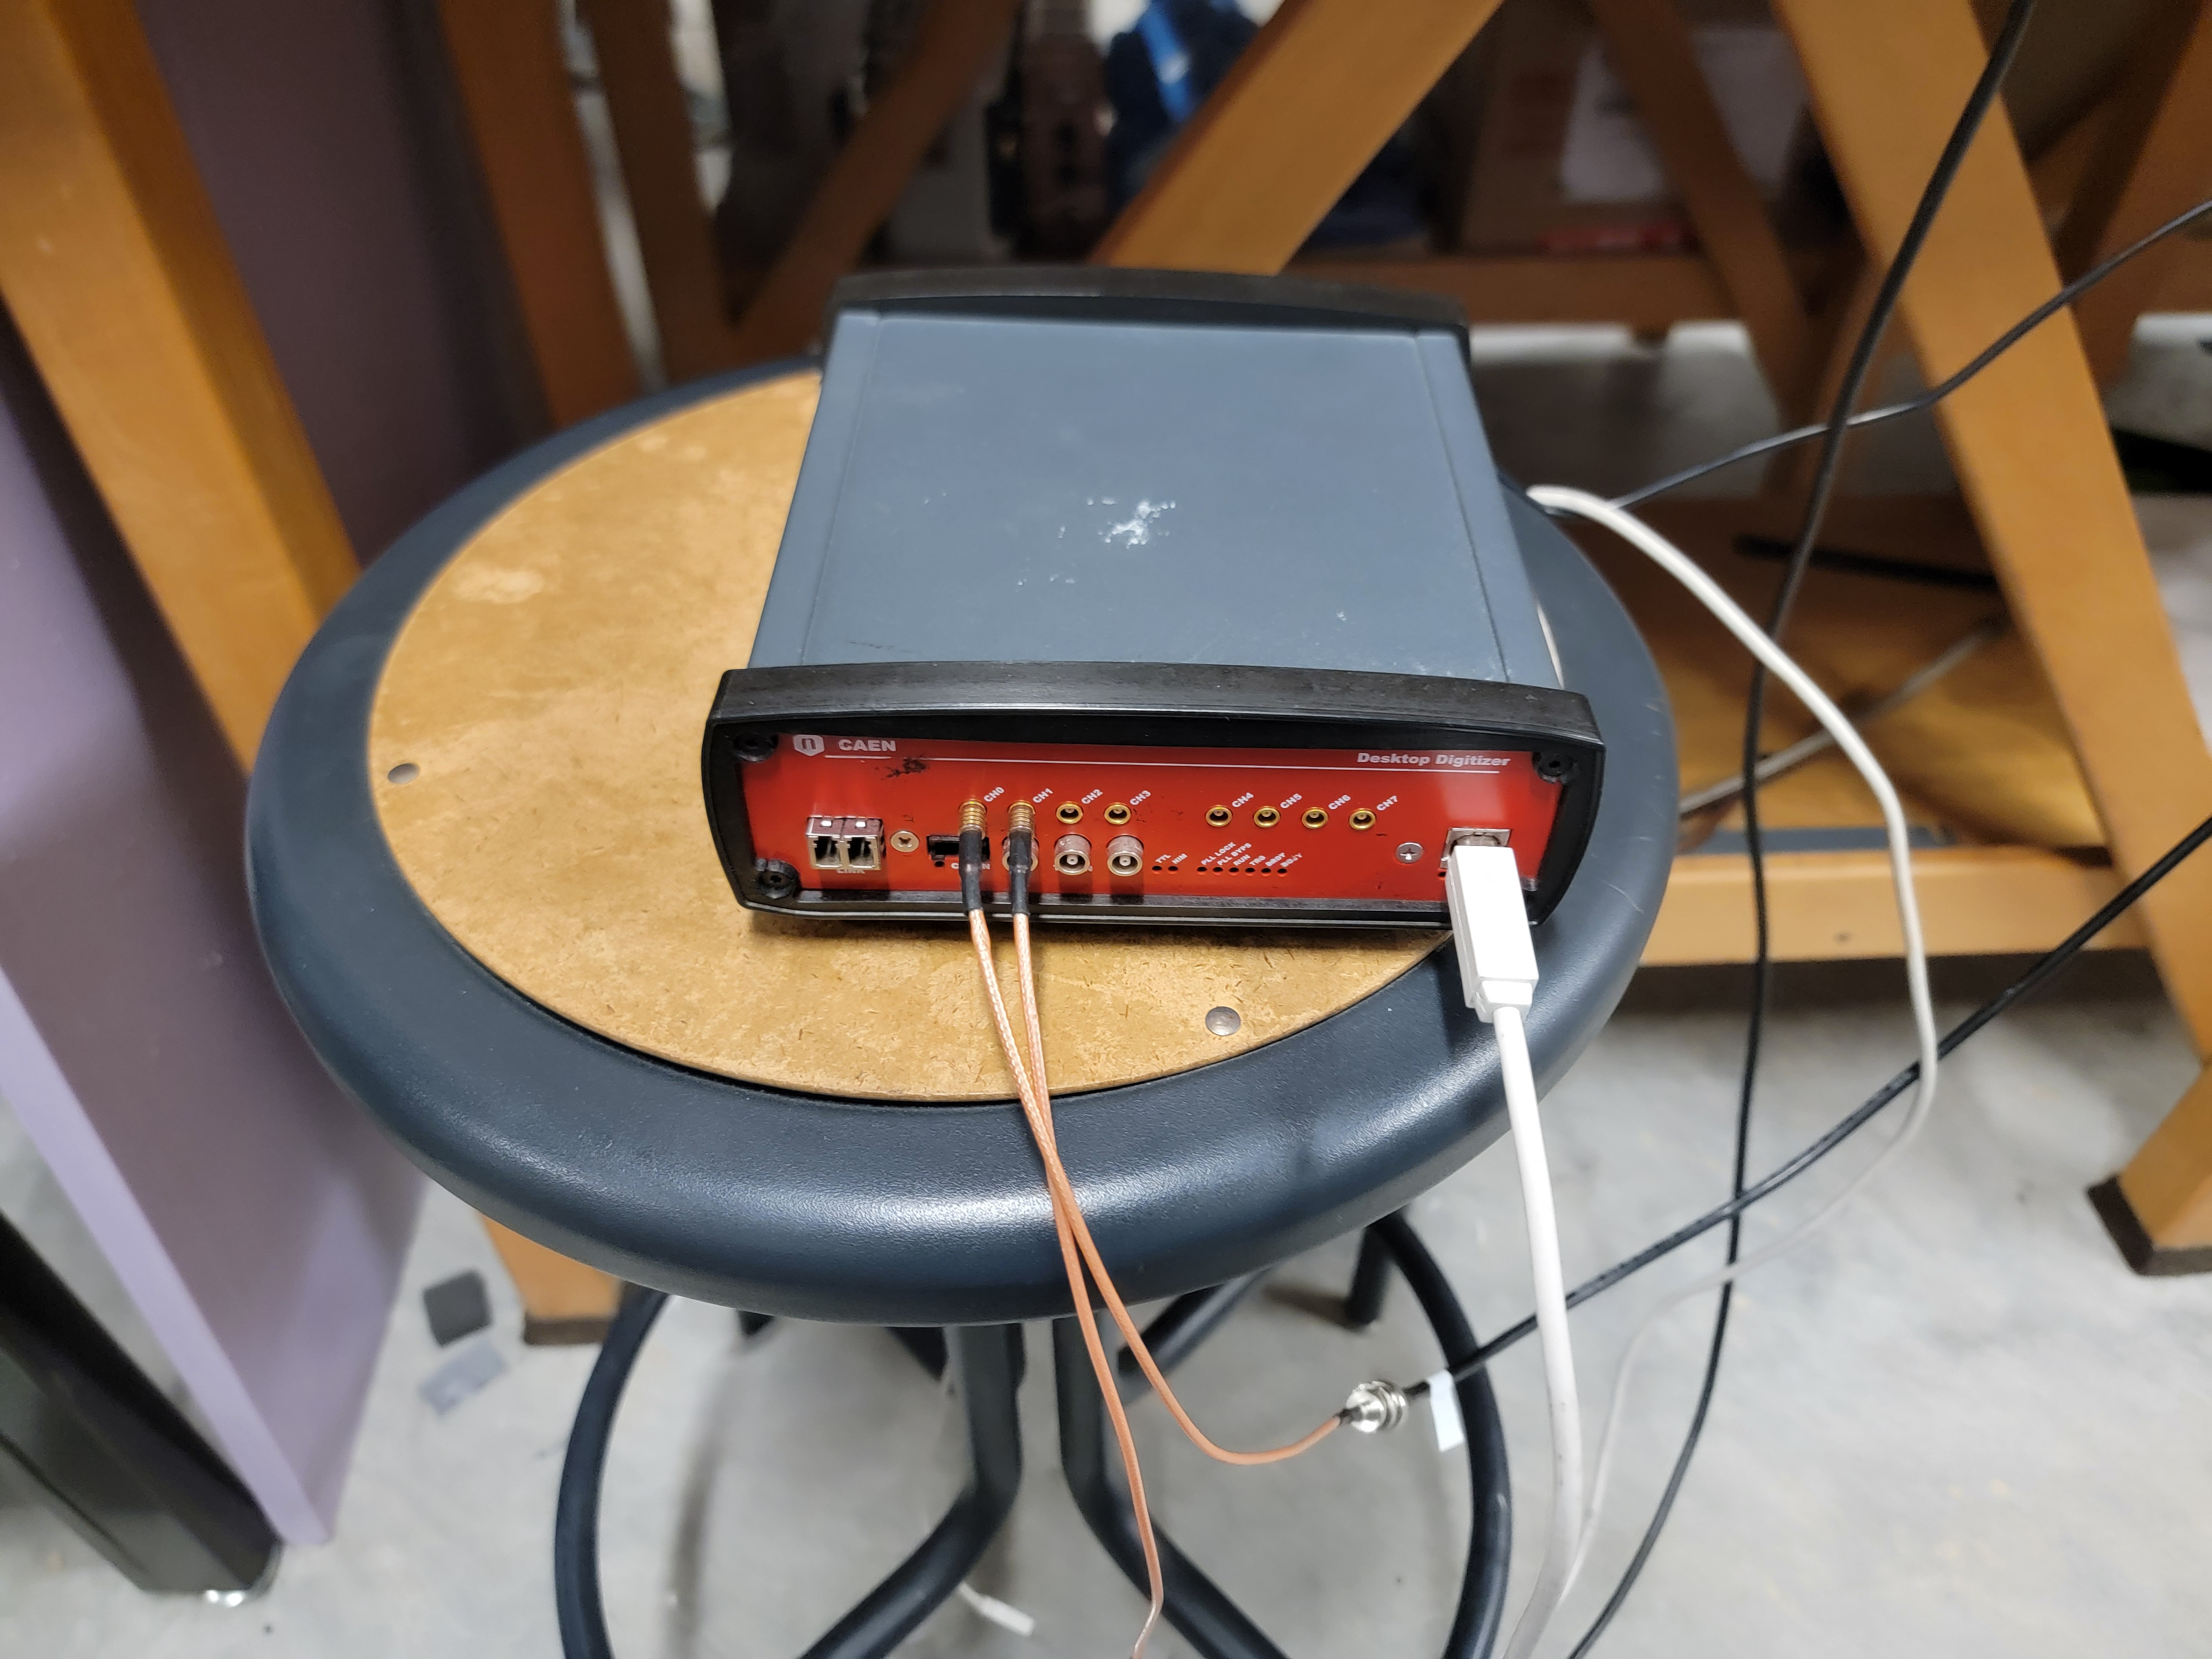
\includegraphics[width=0.6\linewidth]{fig/mat1_digi.jpg}
    \caption{The fast digitizer used in this experiment, with response of the organic scintillator fed into channel 0, response of the inorganic detector fed into channel 1, and output sent through the white USB cable to the laboratory computer.}
    \label{fig:mat1_digi}
\end{figure}

\subsection{Experiment 1: Detector Calibration}

We first connected the stilbene organic detector to the digitzer channel 0 and the HVPS, and applied a negative voltage bias of $-1900$~V to the scintillator.
Placing the \CsSrc source in front of the organic detector, we measured the spectrum of the organic scintillator's response for three~minutes, to use for energy calibration.\\

To record such a spectrum, we opened the computer (connected to the digitizer by USB cable) and started the program Compass, then connected to the digitizer board.
% For data output, we made sure to check the `auto-increment' option (to avoid overwriting files), and to save `Energy' and `$\Delta$T' spectra.\\

We chose input and discrimination settings shown in \figref{fig:set_input} and \figref{fig:set_discrim}; selected (under QDC settings) a gate of 800~ns, short gate of 400~ns, and pre-gate of 48~ns; and selected (under `Onboard coincidences' settings) a coincidence window of 96~ns.
We left `Energy calibration' settings as defaults, as we would later manually calibrate energy of completed spectra.\\

\defplotW{set_input}{The `Input' settings in Compass used for spectrum recordings in this laboratory.}{0.8}
\defplotW{set_discrim}{The `Discrimination' settings in Compass used for spectrum recordings in this laboratory.}{0.8}

After finishing spectrum acquisition, we made sure to reboot the digitizer before measuring the next spectrum.\\


We then connected the NaI(Tl) inorganic detector to the digitizer channel 1 and a different channel of the HVPS, applying a positive voltage bias of $+1350$~V to the inorganic scintillator.\\

Then, moving the \CsSrc source directly in front of the inorganic detector, we repeated the above process to measure the spectrum of the inorganic scintillator's response over three~minutes for calibration.\\

Using predicted features of response spectra in these materials for 661.657~keV gamma rays, we calculated calibration coefficients to use for future spectra of either detector.

\FloatBarrier\subsection{Experiment 2: Angular Compton Scattering Measurement}\FloatBarrier
We then measured Compton scattering at different angles using the coincidence mode of the detector.\\

In Compass, we set operation mode to coincidence mode `Paired AND' with a short time window of 96~ns, to filter for output from the two detectors within such a window of each other.\\

Starting with an angle of 0\degr, we set up the two detectors and the (collimated) gamma source described above to measure Compton scattering at that specific angle (shown in \figref{fig:mat0_setup}).
Ensuring both detectors were properly biased and connected to the digitizer, we recorded the spectrum of coincidental responses from both detectors for 20~minutes in the 0\degr configuration.
We then repeated this recording with the inorganic detector moved to the 30\degr position for 20~minutes, and repeated for the 60\degr and 90\degr positions for 30~minutes each.


\section{Experimental Results}\label{sec:results}
\FloatBarrier

The calibration spectra for the inorganic and organic detectors may be viewed in \figref{fig:dual_cal}.
The spectrum of the inorganic detector (with high-z material) features a prominent photoelectric peak (photopeak) corresponding to the energy of the gamma source (661.657~keV).
The spectrum of the organic detector (with low-z material) does not feature such a photopeak, but we match the edge of the Compton energy range (Compton edge) to the maximum electron transfer energy using Eq.~\ref{eq:comp_max} (477.334~keV).
These calculations found calibration coefficients of 0.252~keV per channel for the inorganic detector, and 1.92~keV per channel for the organic detector.\\

\defplot{dual_cal}{The calibration spectra measured for the organic and inorganic detectors, scaled using known energy values featured in the spectra.}

\FloatBarrier
% Calibration:
% 0.251980198019802~keV/chan for inorganic
% 1.924892774995428~keV/chan for organic

Spectra were successfully measured for scattering targeting the inorganic detector at angles of 0\degr, 30\degr, 60\degr, and 90\degr. 
These spectra can be found in \figref{fig:og_angles_dual} for the organic detector, and in \figref{fig:in_angles_dual} for the inorganic detector, both calibrated using the previously found calibration coefficients.
In the same figures are displayed the theoretical Compton electron and photon energies for each angle, which are included numerically in Table~\ref{tab:comp_E}.

\defplotW{og_angles_dual}{Spectra observed by the organic detector for scattering events at offsets of 0\degr, 30\degr, 60\degr, and 90\degr. Note the correspondence between the peak at each angle, and the predicted Compton recoil electron energy $E_e$.}{0.9}
\defplotW{in_angles_dual}{Spectra observed by the inorganic detector for scattering events at offsets of 0\degr, 30\degr, 60\degr, and 90\degr. Note the correspondence between the peak at each angle, and the predicted Compton photon scatter energy $E_\gamma'$.}{0.9}

\begin{table}[!htb]
    \centering
    \caption{The theoretical Compton electron and photon energies $E_e$ and $E_\gamma'$ corresponding to an incoming photon of energy $E_\gamma=661.657$~keV, with photon scattering angles $\theta$ of 0\degr, 30\degr, 60\degr, and 90\degr, compared to values estimated from observed angular spectra.}
    \label{tab:comp_E}
    \begin{tabular}{c|cc|cc}
        Photon Scattering Angle $\theta$ & $E_e$ (keV) & & $E_\gamma'$ (keV) & \\
         & Predicted & Observed & Predicted & Observed\\\hline
        0\degr & 0 & $40\pm10$ & 661.7 & $590\pm10$ \\
        30\degr & 97.8 & $100\pm10$ & 563.8 & $550\pm10$\\
        60\degr & 260.0 & $230\pm10$ & 401.6 & $410\pm10$\\
        90\degr & 373.3 & $360\pm10$ & 288.3 & $290\pm10$
    \end{tabular}
\end{table}

\FloatBarrier
\section{Discussion}\label{sec:disc}

% The events are linked: the organic detector doesn't have much photopeak so it mostly catches the energy transferred through compton scattering.
% Then, the gamma keeps on going, but if it hits the inorganic detector, which does have photopeak, the inorganic detector can record the energy of that photon. 
% Since the results are linked, this is exactly what we expect: The electron energies which we know correspond to gammas going in a certain angle, have the energy we expect them to.
% The gammas in that angle also have the enrgies we expect them to
% Can now discuss 


The calibration coefficients for the organic and inorganic detectors appear to be self-consistent with each other, as compared in \figref{fig:dual_cal}.
While the organic spectrum lacks a photopeak to compare, the inorganic spectrum has a very muted Compton edge which loosely appears to line up with the theoretical and organic Compton edges, despite not directly being used in the calibration, lending credence to the choice of calibration coefficients.\\

In the angular spectra for the organic detector (\figref{fig:og_angles_dual}), the peaks of energy measured appear to correspond to the predicted energy $E_e$ of Compton recoil electrons from Table~\ref{tab:comp_E}, while in the angular spectra for the inorganic detector (\figref{fig:in_angles_dual}), the peaks of energy appear to correspond to the predicted energy $E_\gamma'$ of the Compton scattered photons.
This is as expected from our experimental design: gamma photons striking the (low-z) organic detector, being Compton scattered in some angle $\theta$.
The organic detector thus detects the Compton electrons and their energy, while the (high-z) inorganic detector, having strong photoelectric response as seen in the calibration curves, produces a response corresponding to that originally scattered photon's energy.\\

While there remain several deviations in these graphs from an ideal expected response, they do not appear to be without explanation.
In both angular spectra sets, substantial broadening of energy occurs, as is expected of any detector, even for a perfectly uniform-energy source.
Our collimation is, additionally, imperfect (still having a somewhat low aperture to length ratio, and lacking the collimation of gamma photons striking the inorganic detector shown in \figref{fig:Lab5_setupnot}), and we would expect a slight additional variation in scattering angles observed from a target angle.
\\

For the angular spectra of the inorganic detectors' response, the background radiation can be observed, but is fairly consistent between angles, making it fairly simple to distinguish between background noise and the peak from scattered Compton photons.\\
The peak in the inorganic 0\degr spectrum appears to fall below the predicted Compton photon energy, while the peak in the same organic spectrum appears to overestimate the predicted Compton recoil electron energy of 0, suggesting the 0\degr measurement was not in taken while perfectly aligned with the collimator.
Between the different angular spectra for the organic detector, we observe remaining traces of a Compton continuum matching the unfiltered calibration spectrum.
This is not unexpected; while we set a tight timing window of 56~ns, it is inevitable that some small number of unrelated Compton electron observations from events unrelated to those reaching the angled inorganic detector were still close enough to either correctly observed photons scattering at that angle, or to unrelated observations by the inorganic detector, to show up on the organic detector's spectra.


\section{Conclusions}\label{sec:conc}

The objectives of the lab were broadly successful. Calibration spectra were successfully measured for the inorganic and organic detectors' responses to 661.657~keV gamma particles, yielding calibration coefficients of 0.252~keV per channel for the inorganic detector, and 1.92~keV per channel for the organic detector.\\

Spectra were successfully measured of the inorganic and organic detectors' responses to Compton scattering of incident 661.657~keV gamma particles at angles of 0, 30, 60, and 90~degrees.
As expected, the peaks measured by the organic detector, which the gamma particles Compton scattered off of, at different angles correspond roughly to the expected Compton electron energy for those angles.
Likewise, the peak energies measured by the inorganic detector oriented towards these angles correspond roughly to the energies expected of Compton photons scattered in these angles.\\

While the angular spectra had some imperfections, their consistency and correspondence with Compton kinematics validates this theoretical model, and future measurements with more precise control of detector angle and collimation, and further optimization of coincidence window, may yield even finer correspondence to this model.\\

This qualified success in selecting for coincidental measurements from two detectors additionally demonstrates the effective use of direct digital acquisition.


% \bibliographystyle{sty/ieeetran}
\pagebreak\printbibliography

\appendix
\pagebreak
\FloatBarrier\section{Equipment Details}\label{app:equip}
In order to better replicate experiments and identify issues, the details of each equipment piece are recorded in Table~\ref{tab:equip}.

\newcommand{\na}{$N/A$}
\newcommand{\sref}[1]{$^{\ref{#1}}$}
\FloatBarrier
Further details of equipment are listed in Table~\ref{tab:equip}.
Where a detail could not be identified for a given device, it is replaced with ``\na''.
\begin{table}[!h]
    \centering
    \small
    \caption{Details of the equipment used in this laboratory.}
    \label{tab:equip}
    \scriptsize
    \begin{tabular}{c|cccc}
        Item & Manufacturer & Model & ID Type & ID Number\\\hline
        % Module rack & Canberra (now Mirion)\sref{addr:mirion}& Model 2000 & Inventory \# & NE759377 \\
        % Geiger-Muller Detector & \na & \na & \na & \na \\
        % GM Pulse Inverter & Spectrum Techniques\sref{addr:spect} & 2017 GPI & \na & \na \\
        % Multichannel Analyzer & Ortec\sref{addr:ortec} & EasyMCA & Inventory \# & P10F79090 \\
        % Alpha Spectrometer & Ortec\sref{addr:ortec} & Model 7401, Si surface barrier detector & Property \# & NE 759377\\
        % Vacuum Pump & Unknown & \na & \na & \na \\
        % Mylar Sheets & Unknown & $5\times3.6$~microns thick & \na & \na \\
        % Aluminum Sheets & Unkown & $5\times18$~microns thick & \na & \na \\
        % Weak Source 1 & Spectrum Techniques\sref{addr:spect} & 1.0\micCi ~$^{137}$Cs Beta Source & Date & Sep. 2017 \\
        % Weak Source 2 & Spectrum Techniques\sref{addr:spect} & 1.0\micCi ~$^{137}$Cs Beta Source & Date & Sep. 2017 \\
        % Strong Source & Eckert and Ziegler\sref{addr:eck-zieg} & 30\micCi~$^{137}Cs$ Beta Source & Date & Sep. 2017 \\
        % \InMeta~Source & \na & Irradiated Indium Foil & Date & Feb. 2026 \\
        Organic Detector & Unknown & Stilbene Scintillator & Unknown & \na \\
        Inorganic Detector & Harshaw\sref{addr:harshaw} & Filtrol NaI(Tl) Scintillator & Unknown & \na \\ 
        Photomultipliers (on detectors) & Ortec\sref{addr:ortec} & Model 276 & Unknown & \na \\
        Fast Digitizer & Caen\sref{addr:caen} & DT5730 / DT5730S & Unknown & \na \\
        Source & Unknown & 30 \micCi \CsSrc & Unknown & \na \\ 
        High Voltage Power Supply & Caen\sref{addr:caen} & N1470AL & Inventory \# & P10G96054 \\
        % Pulser & Ortec\sref{addr:ortec} & Model 480 & \na & \na \\
        % Oscilloscope & Keysight\sref{addr:keys} & Infiniivision DSO-X 2002A & Inventory \# & P10R03513 \\
        % Counter & Ortec\sref{addr:ortec} & Model 871 & Serial \# & 1024 \\
        % Preamplifier & Ortec\sref{addr:ortec} & Model 142PC & Serial \# & 2780r17 \\
        % Amplifier & Ortec\sref{addr:ortec} & Model 590A & Serial \# & 16076205 \\
        Computer & Dell\sref{addr:dell} & Precision 360 & Eng. IT ID \# & EWS 20426 \\

    \end{tabular}
    \begin{enumerate}[label=\alph*]
        % \item\label{addr:mirion}
        % Mirion Technologies, Inc.:
        % 1218 Menlo Drive,
        % Atlanta, GA;
        % Phone: 770.432.2744;
        % \url{https://ir.mirion.com/}
        \item\label{addr:harshaw}
        Harshaw Chemical Company (defunct)
        % \item\label{addr:spect}
        % Spectrum Techniques:
        % 106 Union Valley Rd, Oak Ridge, TN 37830;
        % Phone: 865.482.9937;
        % \url{https://www.spectrumtechniques.com/}
        % \item\label{addr:eck-zieg}
        % Eckert \& Ziegler Isotope Products:
        % 24937 Avenue Tibbitts, Valencia, CA 91355;
        % Phone: +1 866 476-9767;
        % \url{https://isotopeproducts.com/}
        \item\label{addr:ortec}
        Advanced Measurement Technology:
        801 South Illinois Avenue,
        Oak Ridge, Tennessee 37830,
        United States;
        Phone: +1.865.482.4411;
        Fax: +1.865.483.0396;
        \url{https://www.ortec-online.com};
        \item\label{addr:caen}
        Caen Sp.A.:
        Via della Vetraia, 11, 55049 Viareggio LU - Italy;
        Phone: +39 0584 388398;
        \url{https://www.caen.it/}
        % \item\label{addr:keys}
        % Keysight Technologies: 
        % 1900 Garden of the Gods Road, Colorado Springs, CO 80907-3423 United States;
        % Phone: 1 800 829-4444;
        % \url{https://www.keysight.com}
        Email: ortec.info@ametek.com
        \item\label{addr:dell}
        Dell Technologies:
        Dell Technologies
        1 Dell Way
        Round Rock, TX 78664.;
        Phone: 1-877-275-3355;
        \url{https://www.dell.com/en-us/lp/contact-us}
    \end{enumerate}
\end{table}
\FloatBarrier
\end{document}
